% !TEX root = RKWard_paper.tex
\section{Extending RKWard -- an example of creating a plugin}
\label{sec:example_plugin}
As discussed in Section~\ref{sec:technical_plugins}, plugins in RKWard are
defined by four separate files (Figure~\ref{fig:plugin_structure}). To give an impression of the technique,
this section shows (portions of) the relevant files for a plugin that provides
a simple dialog for a t-test. For brevity, the help-file is omitted.

\subsection{Defining the menu hierarchy}
\label{sec:defining_menu_hierarchy}
A so called ``.pluginmap'' file declares each plugin, and, if appropriate, defines where it should
be placed in the menu hierarchy. Usually each .pluginmap file declares many plugins. In this example
we only show one, namely, a two variable t-test (see Figure~\ref{fig:ttest-gui-example}). 
The pluginmap (\code{<!DOCTYPE rkpluginmap>}) gives a unique identifier (``id''), the location of the
GUI description (``file"), and the window title (``label''). The menu layout is defined in a hierarchical
structure by nesting \code{<menu>} elements to form toplevel menus and submenus. Menus with the same ``id''
are merged across .pluginmap files. Moreover, the position within the menu can be explicitly defined (attribute ``index'').
This might be required if the menu entries are to be ordered non-alphabetically.

\begin{footnotesize}
\begin{Code}
<!DOCTYPE rkpluginmap>
<document base_prefix="" namespace="rkward">
  <components>
    <component type="standard" id="t_test_two_vars"
          file="demo_t_test_two_vars.xml" label="Two Variable t-test" />
  </components>
  <hierarchy>
    <menu id="analysis" label="Analysis" index="4">
      <menu id="means" label="Means" index="4">
        <menu id="ttests" label="t-Tests">
          <entry component="t_test_two_vars" />
        </menu>
      </menu>
    </menu>
  </hierarchy>
</document>
\end{Code}
\end{footnotesize}


\begin{figure}[t!]
 \centering
 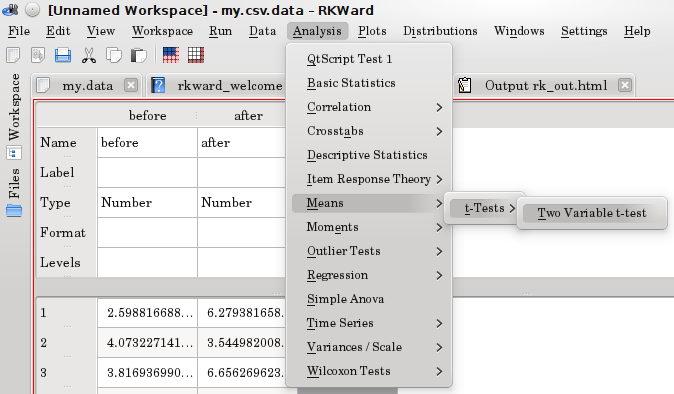
\includegraphics{../figures/ttest-gui-example.png}
 \caption{Generated menu structure as defined by the plugin map.}
 \label{fig:ttest-gui-example}
\end{figure}


\subsection {Defining the dialog GUI}
\label{sec:defining_dialog_ui}
The main \proglang{XML} file of each plugin defines the layout and behavior of the GUI, and references the
\proglang{ECMAScript} file that is used for generating \proglang{R} code from GUI settings and the help file (not included in this paper).

GUI logic can be defined directly in the \proglang{XML} file (the \code{<logic>} element).
In this example, the ``Assume equal variances'' checkbox is only enabled for paired sample tests.
Optionally, GUI behavior can also be scripted in \proglang{ECMAScript}.

The \proglang{XML} file defines the t-test plugin (\code{<!DOCTYPE rkplugin>}) to be organized in two tabs (Figure~\ref{fig:t_test}A).
On the first tab, two variables can be selected (\code{<varslot .../>}). These are set to be ``required'', i.\,e.,
the ``Submit'' button will remain disabled until the user has made a valid selection for both. The second tab includes some
additional settings like the confidence level (default 0.95).

\begin{footnotesize}
\begin{Code}
<!DOCTYPE rkplugin>
<document>
  <code file="demo_t_test_two_vars.js"/>
  <help file="demo_t_test_two_vars.rkh"/>

  <logic>
    <connect client="varequal.enabled" governor="paired.not"/>
  </logic>

  <dialog label="Two Variable t-Test">
    <tabbook>
      <tab label="Basic settings" id="tab_variables">
        <row id="basic_settings_row">
          <varselector id="vars"/>
          <column>
            <varslot type="numeric" id="x" source="vars" required="true"
              label="compare"/>                                                             
            <varslot type="numeric" id="y" source="vars" required="true"
              label="against"/>
            <radio id="hypothesis" label="using test hypothesis">
              <option value="two.sided" label="Two-sided"/>
              <option value="greater" label="First is greater"/>
              <option value="less" label="Second is greater"/>
            </radio>
            <checkbox id="paired" label="Paired sample" value="1" value_unchecked="0" />
          </column>
        </row>
      </tab>
      <tab label="Options" id="tab_options">
        <checkbox id="varequal" label="assume equal variances" value="1"
          value_unchecked="0"/>
        <frame label="Confidence Interval" id="confint_frame">
          <spinbox type="real" id="conflevel" label="confidence level" min="0" max="1"
            initial="0.95"/>
          <checkbox id="confint" label="print confidence interval" value="1"
            checked="true"/>
        </frame>
        <stretch/>
      </tab>
    </tabbook>
  </dialog>
</document>
\end{Code}
\end{footnotesize}

\subsection[Generating R code from GUI settings]{Generating \proglang{R} code from GUI settings}
\label{sec:generating_r_code_from_ui_settings}
A simple \proglang{ECMAScript} script is used to generate \proglang{R} code from GUI settings (using \code{echo()} commands)\footnote{
  See Figure~\ref{fig:t_test}A) for code generated in this example.
}. Generated code for each plugin is divided into three sections: ``Preprocess'', ``Calculate'', and ``Printout'', although each
may be empty.

\begin{footnotesize}
\begin{Code}
var x;
var y;
var varequal;
var paired;

function preprocess () {
  x = getValue ("x");
  y = getValue ("y");

  echo ('names <- rk.get.description (' + x + ", " + y + ')\n');
}

function calculate () {
  varequal = getValue ("varequal");
  paired = getValue ("paired");

  var conflevel = getValue ("conflevel");
  var hypothesis = getValue ("hypothesis");

  var options = ", alternative=\"" + hypothesis + "\"";
  if (paired) options += ", paired=TRUE";
  if ((!paired) && varequal) options += ", var.equal=TRUE";
  if (conflevel != "0.95") options += ", conf.level=" + conflevel;

  echo ('result <- t.test (' + x + ", " + y + options + ')\n');
}

function printout () {
  echo ('rk.header (result\$method, \n');
  echo ('  parameters=list ("Comparing", paste (names[1], "against", names[2]),\n');
  echo ('  "H1", rk.describe.alternative (result)');
  if (!paired) {
    echo (',\n');
    echo ('  "Equal variances", "');
    if (!varequal) echo ("not");
    echo (' assumed"');
  }
  echo ('))\n');
  echo ('\n');
  echo ('rk.results (list (\n');
  echo ('  \'Variable Name\'=names,\n');
  echo ('  \'estimated mean\'=result\$estimate,\n');
  echo ('  \'degrees of freedom\'=result\$parameter,\n');
  echo ('  t=result\$statistic,\n');
  echo ('  p=result\$p.value');
  if (getValue ("confint")) {
    echo (',\n');
    echo ('  \'confidence interval percent\'=(100 * attr(result\$conf.int, "conf.level")),\n');
    echo ('  \'confidence interval of difference\'=result\$conf.int ');
  }
  echo ('))\n');
}
\end{Code}
\end{footnotesize}
